\documentclass{mcmthesis}
\mcmsetup{                     
        tcn = NEUQ001, problem = A,             %% tcn is team control number
        sheet = true, titleinsheet = true,    %% sheet stands for summary sheet
        titlepage = false, abstract = true}    %% titlepage represents abstract page, true or false

%\usepackage{palatino}   
%\usepackage{times}      
\usepackage{txfonts}     



\title{\LaTeX{} Template for MCM/ICM }
\author{\team}
\date{\today}
\begin{document}

\begin{summary}
The 2014 Ebola virus (EBOV) outbreak in West Africa is so far the largest and
deadliest recorded in history. It is thus crucial to better understand the spread
of infection and to mitigate the outbreak in the affected countries.

We describe the epidemic using a delayed SEIQR
(susceptible-exposed-infective-quarantined-removed) model.
We fit the model to the most recent reported data of infected cases and deaths in Sierra Leone and Liberia.
To aid in planning for additional disease-control efforts,
we introduce Ebola treatment units (ETU) and pulse vaccination in this model.
We find that the EBOV epidemic begins to decrease and eventually end if people with Ebola
virus can be isolated in ETUs with medical care.

Based on the SEIQR model, we cluster the affected areas with Self-Organizing Map (SOM) neural network.
We then formulate a multi-layer dynamic drug distribution model incorporating the results of the SOM
clustering, which contributes significantly in controlling epidemic areas with
relatively high degree of urgency. With the goals of minimizing the
transportation cost and decreasing the unsatisfied demand for the urgency
logistics network, we employ the artificial immune system (AIS) to locate the
distribution center.chinatex

The main advantage of our approach is that the models utilize clever
algorithm allowing us to see clearly how preventions and interventions can
mitigate and eventually stop the epidemic. A limitation of our approach is
that we constrict the population flow within countries and underlie national
epidemic transmission. Results of our models not only support the
construction of a medical material delivery system, but also demonstrate the
needs for more ETUs to be established, supplied, and staffed.

\noindent
\textbf{Key Words:}
SEIQR Model; Self-Organizing Maps; Immune Algorithm; Deliver System;

\end{summary}


\maketitle



%\newpage
%\thispagestyle{empty}
%\begin{center}
%\bfseries\Large
%Synopsis/Memo/Handout
%\end{center}
%
%This is Synopsis/Memo/Handout.




\thispagestyle{empty}
\newpage
\tableofcontents
\newpage
\setcounter{page}{1}
\section{Introduction}

\subsection{Restatement of problems}


\begin{itemize}
\item minimizes the discomfort to the hands, or
\item maximizes the outgoing velocity of the ball.
\end{itemize}
We focus exclusively on the second definition.

\begin{itemize}
\item the initial velocity and rotation of the ball,
\item the initial velocity and rotation of the bat,
\item the relative position and orientation of the bat and ball, and
\item the force over time that the hitter hands applies on the handle.
\end{itemize}

\begin{itemize}
\item the angular velocity of the bat,
\item the velocity of the ball, and
\item the position of impact along the bat.
\end{itemize}

\emph{center of percussion} [Brody 1986],



%=======
\begin{Theorem} \label{thm:latex}
\LaTeX
\end{Theorem}

\begin{Lemma} \label{thm:tex}
\TeX .
\end{Lemma}

\begin{proof}
The proof of theorem.
\end{proof}


\subsection{Other Assumptions}
D. E. Knuth \cite{Knuth},
the author of \textit{the Art of Computer Programming},
is a very famous computer scientist,
now living at Stanford University.




\section{Analysis of the Problem}

%LaTeX²åͼָÄÏ
\begin{figure}[ht]
\label{fig:aa}
\small
\centering
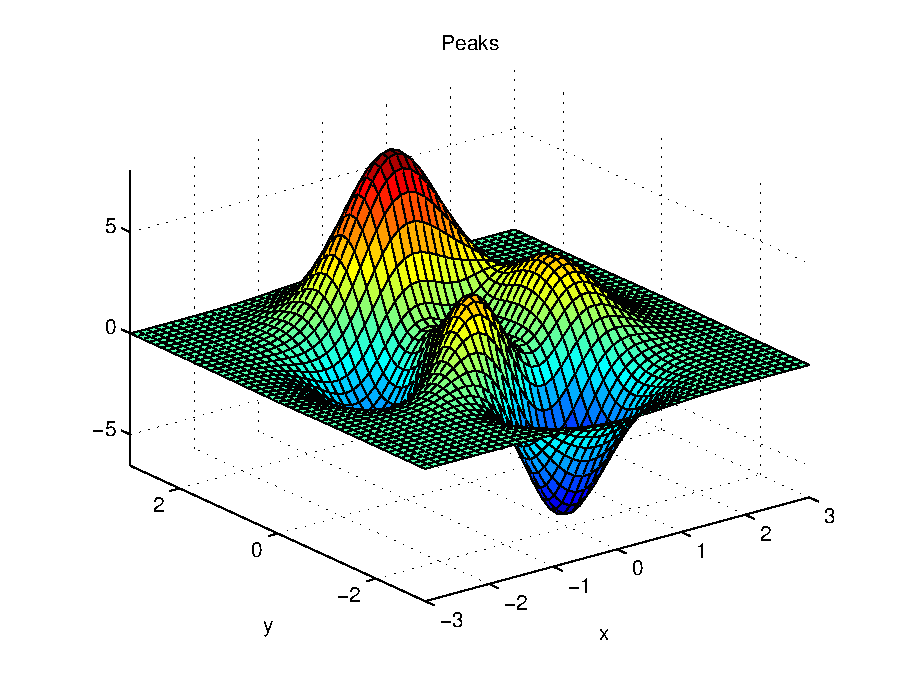
\includegraphics[width=12cm]{mcmthesis-aaa.eps}
\caption{The Curve Plane of System}
\end{figure}

%1£¬²»ÒªÓÃ×Óͼ£¬subfig£¬subfigure¡£
%2£¬¾¡Á¿¼õÉÙ¸¡¶¯»·¾³£¬Í¼¾¡Á¿£¬ËõСͼµÄռλ

It follows that
\begin{equation}\label{aa}
a^2 + b^2 = c^2
\end{equation}


The equation \eqref{aa} has told that

\[
\begin{pmatrix}
  a_{11}  & a_{12}  & a_{13}   \\
  a_{21}  & a_{22}  & a_{23}   \\
  a_{31}  & a_{32}  & a_{33}
\end{pmatrix}
= \frac{{Opposite}}{{Hypotenuse}}\cos^{-1} \theta \arcsin \theta
\]

\[
p_{j}=
\begin{cases}
0,             & \text{if $j$ is odd}\\
r!\,(-1)^{j/2},& \text{if $j$ is even}
\end{cases}
\]



\[
\arcsin \theta  = \oint\limits_\varphi \lim_{x \to \infty } \frac{n!}{r! (n - r)!} \eqno (23)
\]

\section{Calculating and Simplifying the Model  }

Calculating and simplifying the model:

\section{The Model Results}
\begin{table}\caption{A three-line form}
\begin{center}
\begin{tabular}{p{80pt}p{80pt}p{80pt}}
\toprule
sysmtem     & Version & Editor \\
\midrule
Windows     & Mik\TeX  & \TeX{}MakerX \\
Unix/Linux  & te\TeX   & Kile \\
\bottomrule
\end{tabular}
\end{center}
\end{table}


\section{Validating the Model}




\section{Evaluate of the Mode}

\section{Strengths and weaknesses}


\subsection{Strengths}
\subsection{Weaknesses}

\section{Conclusions}
\begin{itemize}
\item \textbf{Applies widely}\\
This  system can be used for many types of airplanes, and it also
solves the interference during  the procedure of the boarding
airplane,as described above we can get to the  optimization
boarding time.We also know that all the service is automate.
\item \textbf{Improve the quality of the airport service}\\
Balancing the cost of the cost and the benefit, it will bring in
more convenient  for airport and passengers.It also saves many
human resources for the airline.
\end{itemize}














\begin{thebibliography}{99}
\bibitem{Knuth} D.~E. Knuth.  The \TeX{}book,
the American Mathematical Society and Addison-Wesley Publishing Company, 1984-1986.

\bibitem{Lamport}
Lamport, Leslie.  \LaTeX{}:``A Document Preparation System'',
Addison-Wesley Publishing Company, 1986.

\bibitem{latex}
http://www.latexstudio.net/


\bibitem{chinatex}
http://www.chinatex.org/

\end{thebibliography}

%\hspace{2em}
\begin{appendices}

\section{First appendix}

Here are simulation programmes we used in our model as follow.\\

\textbf{\textcolor[rgb]{0.98,0.00,0.00}{Input matlab source:}}
\lstinputlisting[language=Matlab]{./code/mcmthesis-matlab1.m}

\section{Second appendix}

some more text \textcolor[rgb]{0.98,0.00,0.00}{\textbf{Input C++ source:}}
\lstinputlisting[language=C++]{./code/mcmthesis-sudoku.cpp}

\end{appendices}
\end{document}
